% ex: tw=74 ts=4 sw=4
\documentclass{article}
\usepackage[utf8]{inputenc}
\usepackage[normalem]{ulem}
\usepackage{amsmath}
\usepackage{xkeyval}
\usepackage[bookmarksnumbered]{hyperref}
%\hypersetup{pdfborder=0 0 0}
\usepackage{multirow}
\usepackage{todonotes}
\usepackage[english]{babel}
\usepackage{tabulary}
\usepackage{tabularx}
%\usepackage{fullpage}
%\usepackage{natbib}
\usepackage[all]{hypcap}

\newcommand{\wire}{\texttt}

\title{802.16-2009 OFDM PHY - Digital Realm Transmitter Implimentation}
\author{Cody Schafer}
\date{\today}
\begin{document}
\maketitle


\section{Project Overview}
We are developing a minimal 802.16-2009 OFDM Transmitter PHY.  This PHY
supports only QPSK-1/2 modulation-convolution rate. Additionally, any
components not relevant to unlicensed bands are omitted.  All optional items
are omitted.

This PHY requires the cooperation of a MAC layer implementation which is
compliant with the 802.16-2009 standard in order for the compliance
expectations (\autoref{sec:comply}) to be met.

\begin{wrapfigure}{r}{0.5\textwidth}
\begin{center}
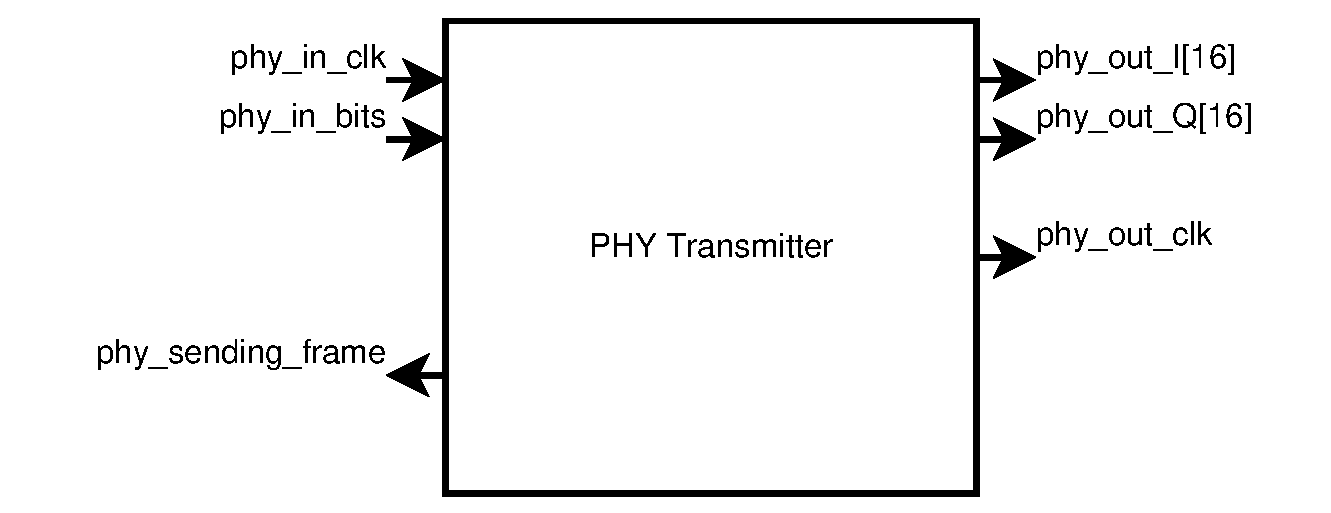
\includegraphics[width=0.48\textwidth]{t_block}
\caption{Overall Transmitter Interface}
\label{fiig:all-blockl}
\end{center}
\end{wrapfigure}

\begin{comment}
\todo[inline]{Derive the product from the needs}
\end{comment}

	\subsection{End Market Expectations}
	Currently IEEE 802.16, also known as ``WiMAX'', has seen little
	deployment in the United States and western Europe while being
	moderately deployed in Asian nations and Eastern European markets.
	To be useful in western areas, WiMAX has to effectively compete
	with both consumer owned Wifi hot-spots and the various cell phone
	networks. Given the impressively low cost of both cellular and Wifi
	(802.11) systems combined with the expectation that they work well
	in mobile devices, this physical layer (PHY) targets both
	simplicity (to reduce cost) and reduced power consumption.

	\subsection{Degree of standards compliance and scope limitations}
	\label{sec:comply}
	The 802.16 standard specifies multiple layers of a WiMAX device,
	including a ``Service-specific convergence
	sublayer''~\cite[section 5]{IEEE:802.16}, a MAC
	sublayer~\cite[section 6]{IEEE:802.16}, a Security
	sublayer~\cite[section 7]{IEEE:802.16}, and the Physical
	layer~\cite[section 8]{IEEE:802.16}. 
	
	The PHY, while being described within section 8 of the 802.16-2009
	document, is additionally subject to certain constraints and
	requirements stipulated within the other sections.  These sections
	where only utilized to the extent to which they apply to design of
	the PHY component.

	Applicable sections of \cite{IEEE:802.16}.
	\begin{itemize}
		\item Section 8.3 - OFDM description
		\item Section 8.3.3.4.1 - Data Modulation: implementation
			is not compliant with this section, only QPSK
			modulation is supported.
		\item 8.3.3.4.3 - Rate ID encodings: not compliant with
			this section, only the QPSK-1/2 rate ID is supported.
		\item 8.3.5.1.1 - DL subchannelization: Rate ID
	\end{itemize}

\section{Electrical Characteristics}
All voltages of logic levels are defined by the FPGA on which the product's
code is placed.

\todo[inline]{Need these defined}

\section{OFDM Parameters}

\subsection{Primitive Parameters}

\begin{description}
	\item[BW]: This is the nominal channel bandwidth.
	\item[$N_{used}$]: Number of used subcarriers.
	\item[n]: Sampling factor. This parameter, in conjunction with BW
		and $N_{used}$ determines the subcarrier spacing, and the
		useful symbol time.
	\item[G]: This is the ratio of CP time to ``useful'' time.
\end{description}


\todo[inline]{Insert a table of the values that are fixed by the standard and our
implimentation limitations}

\subsection{Derived Parameters}

\begin{description}
	\item[$N_{FFT}$]: Smallest power of two greater than $N_{used}$
	\item[Sampling Frequency]: $F_s = floor ( n \cdot BW / 8000 )
		\times 8000 $
	\item[Subcarrier spacing]: $\Delta f = F s / N_{FFT} $
	\item[Useful symbol time]: $T_b = 1 / \Delta f$
	\item[CP Time]: $T_g = G \cdot T_b$
	\item[OFDM Symbol Time]: $T_s = T_b + T_g$
	\item[Sampling time]: $T_b / N_{FFT}$
\end{description}

\todo[inline]{Tables of valid values for each of the derived values}

\section{External Interface to the PHY Transmitter}
\label{sec:frame}
The MAC interfaces with the PHY module by sending frames (with the
appropriate headers and padding included) as a stream of bits.  These bits
are clocked via the \textbf{mac\_clk\_in} line, and must only be sent when
the \textbf{mac\_sending\_frame} line is high.  The state of the
\textbf{mac\_sending\_frame} line must be low when not sending a frame, and
must be lowered and raised between frames that would otherwise be abutting.
The frequency of \textbf{mac\_clk\_in} must be less than or equal to half
of the \textbf{phy\_clock}.

The \textbf{phy\_ready} line is a signal to the mac that it is ready for a
new frame to be inputed, and should not be ignored.

The structure of individual frames detailed in section 8.3.5 of IEEE
802.16-2009.  Each frame contains a header, up to 4 DL sub-frames (each with
their own structure also defined in IEEE802.16-2009 section 8.3.5) and some
number of UL sub-frames.  Note that due to fixing certain implementation
parameters, some fields are constrained further than mentioned within the
standard.

\begin{description}
	\item[Frame Header - Rate\_ID] is fixed at '1' indicating QPSK
		modulation with a code rate of $1 over 2$.
	

\end{description}
\todo[inline]{Determine Full inputs and outputs}

\begin{table*} \begin{tabularx}{\linewidth}{c|c|c|X}
	\label{tbl:extern-io}
	Name & Width & Direction & Description\\ \hline

	\wire{phy\_out\_I} & 16 & O & The real component of the output,
	clocked by \wire{phy\_out\_clk} \\

	\wire{phy\_out\_Q} & 16 & O & Imaginary component of the output,
	clocked by \wire{phy\_out\_clk} \\

	\wire{phy\_out\_clk} & 1 & O & Clocks out the I and Q values
	produced by the PHY. \\

	\wire{phy\_in\_bits} & 1 & I & Input bitstream from a MAC
	device. \\

	\wire{phy\_in\_clk} & 1 & I & Clock at which the input bitstream
	\wire{phy\_in\_bits} should be sampled. \\

	\wire{phy\_in\_frame} & 1 & I & Set low while the current set of
	bits is from the same frame. Must be set high for one clock cycle
	between frames. \\

	\wire{bsid} & 4 & I & The lower four bits of the BSID, a unique
	identifier. \\
	
	\wire{bw} & 3 & I & Channel bandwidth. See \autoref{tbl:bw}. \\
\end{tabularx}
\caption{External Interface to the PHY transmitter.}
\end{table*}

\begin{table} \begin{center} \begin{tabular}{c|c}
	\label{tbl:bw}
	
	\wire{bw[3]} & Bandwidth in MHz \\ \hline

	0 & 1.25 \\
	1 & 1.5  \\
	2 & 1.75 \\
	3 & 2.0  \\
	4 & 2.75 \\
	5 - 7 & Undefined

\end{tabular} \end{center} \caption{Meanings of BW values.} \end{table}

\section{Internal Interfaces}
This section covers the interfaces for internal structures within the PHY
transmitter which are not exposed for use by the MAC or any other interfacing
hardware.

\autoref{tbl:internal-common-wire} shows some of the common signals for
the internal interfaces.

\begin{table*}
\begin{tabulary}{\linewidth}{c|C|L}
	\label{tbl:internal-common-wire}
	Name & Active Level & Meaning \\ \hline
	
	\wire{*\_valid} & high & Indicate the source outputting the signal
	is also outputting data (clocked via the \wire{phy\_clock}) which
	should be processed by the next item in the chain. \\

	\wire{*\_bits} & high & A serial stream of bits clocked by
	\wire{phy\_clock}. Only valid when the corresponding
	\wire{*\_valid} line is also active. \\

	\wire{*\_flag} & high & Set active for a single clock cycle
	before becoming inactive again.
\end{tabulary}
\caption{Common signals used internally}
\end{table*}

Each block of the transmitter connected via direct wiring (without a
buffer) is given the same clock. Each block reads its inputs on alternating
clock edges such that two adjacent units read and write on different edges.
This is done so that outputted data does not change while being read.

%% FRAME
%% BURST

\todo{see planned.tex}

%% RAND
 
\todo{see impl/rand.tex}

%% FEC

\todo{see impl/reed-solomon.tex}

%% FEC TO INTERLEAVER


%% INTERLEAVER

\todo{See impl/interleave.tex}

% CONSTELLATION MAPPING
% IFFT INPUT BUFFER.

% IFFT
% CYCLIC PREFIX

\todo{See planned.tex}

\section{Testing Considerations}
\section{Economic Analysis}
\section{Power Consumption}
\section{FPGA Implementation}
  \subsection{Sampling and Clock Rate}
    From the IEEE 802.16 standards document, the sampling rate for
    256-OFDM is defined as
    \begin{equation}
    F_s = BW * 7/6
    \end{equation}
  
  \begin{center}
  \begin{tabular}{c|c}
  Channel Bandwidth & Sampling Rate \\ \hline
  14 MHz & 16.333 MHz \\
  7 MHz & 8.166 MHz \\
  3.5 MHz & 4.083 MHz \\
  1.75 MHz & 2.042 MHz
  \end{tabular}
  \end{center}
  
  This design should be able to run on both the Spartan-3 FPGA and Virtex 4 LX60
  FPGA as they both supply a 500 MHz clock.
  
  \subsection{Power Calculation}
  
  Calculate power based on required clock frequency for the device as well as the
  FPGA specifications for voltage inputs.
  
  Absolute Maximum rating for $V_{in}$ : 4.4 V
  
  Clock frequency required for a 3.5 MHz channel bandwidth : 4.083 MHz
  
  Input capacitance over recommended operating conditions : 10 pF
	%Input capacitance per input pin?
  \begin{center}\begin{equation}
  P = C * V^2 * f = 10 pF * (4.4 V)^2 * 4.083 MHz = 0.18 mW
  \end{equation}\end{center}
  \todo[inline]{Is this correct?}
  
	%\subsection{Pin outs}
	%XC3S200-FT256
	%//Top and Bottom View Package FT256 -   %http://www.xilinx.com/support/documentation/package_specs/ft256.pdf 
	%\section{Datasheet(Spartan-3 FPGA}
	%\subsection{Electrical Characteristics}
	%\begin{tabular}
	%\end{tabular}


\end{document}
